\documentclass[11pt,a4paper]{article}
\usepackage[T1]{fontenc}
\usepackage[a4paper,margin=2.2cm,top=2.5cm,bottom=2.4cm,headheight=14pt]{geometry}
\usepackage{booktabs}
\usepackage{array}
\usepackage{xcolor}
\definecolor{accent}{RGB}{30,64,175}
\definecolor{ink}{RGB}{31,41,55}
\usepackage{tikz}
\usetikzlibrary{arrows.meta}
\usepackage{fancyhdr}
\usepackage{float}
\usepackage[colorlinks=true,linkcolor=accent,urlcolor=accent,citecolor=accent]{hyperref}

\newcolumntype{L}[1]{>{\raggedright\arraybackslash}p{#1}}
\newcolumntype{R}[1]{>{\raggedleft\arraybackslash}p{#1}}
\setlength{\parindent}{0pt}
\setlength{\parskip}{5pt}

\pagestyle{fancy}
\fancyhf{}
\fancyhead[L]{\small\color{ink} AuditIQ: project overview}
\fancyhead[R]{\small\thepage}
\renewcommand{\headrulewidth}{0.4pt}

\begin{document}

% ----------------------------------------------------------------- title page
\thispagestyle{empty}
\vspace*{1.5cm}
\begin{center}
{\fontsize{30}{34}\selectfont\bfseries\color{accent} AuditIQ}\\[6pt]
{\Large Project overview: extra features, architecture and status}\\[14pt]
Major project, phase 1\\[10pt]
{\large Chandana Devanaboyina \qquad Podichetty Samiksha \qquad Medapally Shiva Reddy}\\[4pt]
{\small Department of Information Technology, Chaitanya Bharathi Institute of Technology, Hyderabad}\\[14pt]
{\small Status as of 18 October 2026}\\
{\small Repository \url{https://github.com/Chandana909/major.project}, branch \texttt{main}}
\end{center}
\vspace{1.2cm}

\noindent\textbf{About this document.} This document describes what AuditIQ is, what this phase has built, how the system is organised, and which results have been measured. It is written for the project team and for reviewers. Every number in it is read from a file that a script of the repository writes; the table or the text that uses it names that script. Expected values are targets fixed before measurement, and are labelled as expected. The language-model stages have been run only on samples (20 and 34 invoices), and the text says so wherever it matters. The full list of results, with every source file, is \texttt{RESULTS.md} at the root of the repository.

\newpage
{\footnotesize\renewcommand{\addvspace}[1]{}\tableofcontents}
\newpage

% ---------------------------------------------------------------- 1 summary
\section{Summary}
AuditIQ checks procurement invoices for forensic audit and compliance. For each invoice it gathers the purchase order, the goods receipt, the vendor record, the approval log and the vendor's other invoices, checks them against a written policy, and recommends whether the invoice can be paid without review, must be sampled, or must be reviewed. Every decision keeps its findings, the evidence each finding quotes, the policy clause it cites with its document and page, and a trail of every step.

The base system is a multi-agent pipeline that follows two published works: AuditBench~\cite{wang2025auditbench}, which measures how well large language models audit financial statements, and a survey of large language model based multi-agent systems in financial markets~\cite{liu2026survey}. The central extra feature is \emph{policy-driven deterministic controls}. The organisation's policy document configures the checks. The system reads the policy PDF, takes every threshold from the wording of the rule that states it, and twelve deterministic controls execute those thresholds before any language model is called. No threshold is typed into code or into a prompt.

Around this feature the project built five more capabilities: policies written in free prose can be read by a model whose proposals code verifies and a named person confirms; reviewers decide invoices with a forensic trail; a REST API and a web application show the results, including three three-dimensional views; a copilot answers with citations; and an evaluation harness produces every number the project reports.

\begin{table}[htbp]
\caption{The key results, all measured by scripts of the repository}
\label{tab:key}
\centering
\small
\begin{tabular}{L{5.2cm}L{10.5cm}}
\toprule
Question & Result \\
\midrule
Does the audit follow a changed policy? & 196 of 196 threshold values and 224 of 224 rules were read correctly from 14 policy documents; the policy-driven controls made 0 wrong decisions in 560,000 audits. On 20 held-out random documents: 280 of 280 values, 0 wrong decisions in 800,000 audits. \\
Does the reader refuse what it cannot execute? & 16 edited documents: 7 of 7 harmless edits read correctly, 9 of 9 defective or ambiguous documents refused with the reason. \\
How wrong is a system whose thresholds are not updated? & Up to 30.7\% of 40,000 invoices were decided against the policy in force (the strict policy). \\
How do the controls compare with classical detectors? & F1 0.833 at precision 1.000, against 0.536 for an isolation forest and 0.498 for a one-class SVM, on three ledgers of 5,000 invoices. \\
Can a model read a policy written in its own words? & 80 of 84 values were proposed correctly for six documents. The code check verified 56, held back 24 correct values, caught 2 wrong values and passed 2. \\
How fast is the control stage? & About 18 $\mu$s per invoice; 172,226 invoices per second with eight processes on one laptop. \\
How do the language-model stages do? & On 34 invoices of a benchmark ledger the agents found 12 of 20 judgement anomalies, and 0.375 of their findings named the violated rule; the single prompt found 4 and 0.031. A sample: no difference is significant. \\
\bottomrule
\end{tabular}
\end{table}

% ------------------------------------------------------------- 2 what we do
\section{What we are doing}
\subsection{Aim}
A procurement audit has to establish, for every invoice, that it matches an approved purchase order, that the goods or services were received, that the vendor is legitimate and tax-compliant, and that the payment was approved within the approver's limit. The rules that define exceptions are written in an organisation-specific policy document. When the policy changes, a system whose thresholds are typed into code or prompts has to be edited by hand, and nothing shows that the edit agrees with the document. AuditIQ is built so that the policy document is the configuration of the audit, and so that every decision can show the rule, the evidence and the page it rests on.

\subsection{The question the paper answers}
\begin{quote}
When an organisation changes its policy and supplies only the new document, does the system decide every invoice as the new policy requires, and how wrong is a system that is not updated?
\end{quote}

\subsection{Contributions}
\begin{itemize}
\item \textbf{Policy as data.} Thresholds are read from the policy PDF into a clause registry, which twelve controls execute. A document that cannot be executed is refused, with the reasons.
\item \textbf{A measured answer to the question}: the adherence of the policy-driven controls, and the error of a frozen system, on fourteen policy documents.
\item \textbf{A reading path for policies in their own wording}, in which a model proposes, code verifies and a named person confirms. Nothing is stored unverified.
\item \textbf{A complete platform around these}: the audit pipeline with its configurations, a review workflow with a forensic trail, a REST API, a web application, a copilot and an evaluation harness, all tested and under continuous integration.
\end{itemize}

\subsection{Work in this phase}
The work follows the plan of the project, in four parts.

\begin{table}[htbp]
\caption{The parts of the project and their status on 18 October 2026}
\label{tab:phases}
\centering
\small
\begin{tabular}{L{1.5cm}L{6.6cm}L{7.2cm}}
\toprule
Part & Content & Status \\
\midrule
A & Work that needs no model: datasets, controls, classical baselines, policy reading, policy change, scalability, policy search. & Done and measured (Section~\ref{sec:measured}). \\
B & The language-model pipeline: specialist agents, challenger, agreement re-runs, configurations C1 to C5, batch runner. & Built and tested with a scripted model. Run with a local 7B model on a pilot of 20 invoices and on a sample of 34 invoices of benchmark ledger 101. Full benchmark ledgers wait for a faster model endpoint. \\
C & The application: the database on SQLite and PostgreSQL, the review queue and decisions, policy adoption, the copilot, the Streamlit dashboard, the REST API, the web application with 3D views, and loading a ledger from Excel or a zip archive. & Built. 330 Python test cases and 28 frontend tests. Continuous integration passes. All seven pages were checked in a browser. \\
D & The paper: measured results, expected values, references. & Updated to 13 pages, with the held-out, robustness and benchmark-sample results. It waits for the team's review and for the template of the target venue. \\
\bottomrule
\end{tabular}
\end{table}

\subsection{Open decisions and items}
\begin{table}[htbp]
\caption{Decisions and items that the team has to settle}
\label{tab:open}
\centering
\small
\begin{tabular}{L{6.2cm}L{3.0cm}L{6.1cm}}
\toprule
Item & Who & Status \\
\midrule
A model endpoint for configurations C2 to C5 on the benchmark: a GPU or a hosted open-weight model. & Team & Open. It decides when the benchmark runs can be made. \\
Near-duplicate invoices (class J1): make them a rule-defined class with a control for rule 2.2.2 (recommended), or keep them as a judgement class. & Team & Open. \\
The old database password, written in the reference folder. & Owner of the old database & Open. It should be rotated. The folder is excluded from git. \\
The third author's affiliation and contact. & Team & Assumed to be the same department; to be confirmed. \\
The target venue's template and page limit. & Team & Unknown. The paper is 13 pages in the IEEEtran conference format. \\
The two base papers, read in full. & Team & Open. Section III of the paper agrees with both published abstracts; the full texts are behind the Springer paywall and must be read through the college library. \\
\bottomrule
\end{tabular}
\end{table}

\subsection{Relation to the earlier prototype}
The earlier hackathon prototype is kept in the reference folder AuditIQ-DeloitteHacksplosion-main. It was built with Flowise and holds a hard-coded database credential. AuditIQ is a standalone system: it does not use the Flowise flows, and the reference folder is excluded from the repository. The features in Section~\ref{sec:features} are those of the standalone system.

% ----------------------------------------------------------- 3 architecture
\section{Architecture}
\label{sec:arch}
\subsection{Layered view}
AuditIQ is built in five layers (Figure~\ref{fig:layers}). The interfaces show the work to people. The REST API is the only route by which the web application reaches the system. The application services hold the logic. The data store keeps every fact the system uses or produces. The external services are the language models and the policy documents. The interfaces call the same modules as the command line, so a decision taken in the browser is the decision the command line would take. The web application and the API are built with React~\cite{r3f}, three.js~\cite{threejs} and FastAPI~\cite{fastapi}; the pipeline is a LangGraph~\cite{langgraph} state graph; policy PDFs are read with PyMuPDF~\cite{pymupdf}.

\begin{figure}[htbp]
\centering
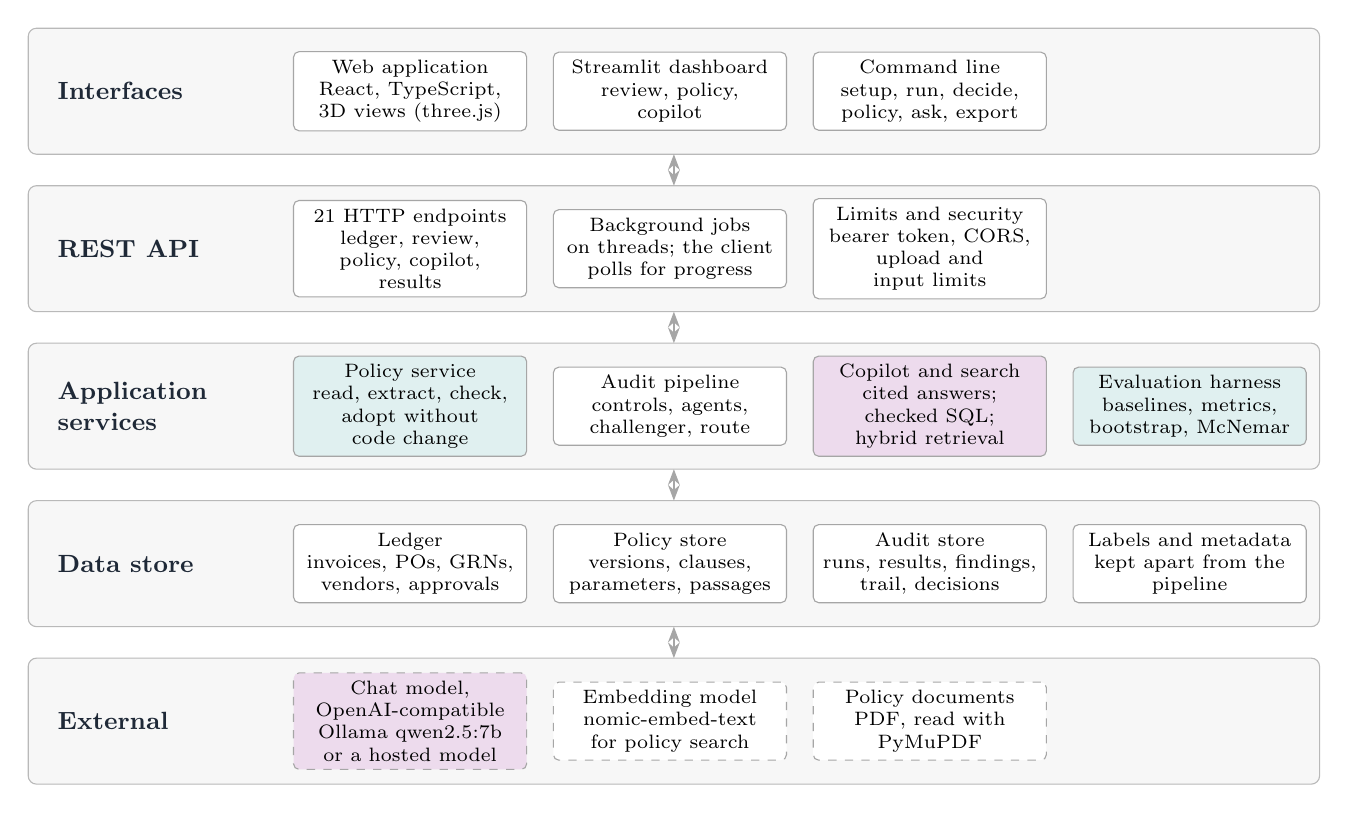
\begin{tikzpicture}[
  layer/.style={draw=gray!55, fill=gray!6, rounded corners=3pt, minimum width=16.4cm, minimum height=1.6cm},
  comp/.style={draw=gray!70, rounded corners=2pt, fill=white, align=center, font=\scriptsize, text width=2.75cm, inner sep=3pt},
  code/.style={comp, fill=teal!12},
  llm/.style={comp, fill=violet!14},
  ext/.style={comp, dashed},
  lab/.style={font=\small\bfseries, text=ink, align=left, text width=2.5cm, anchor=west},
  arr/.style={<->, >={Stealth[length=2mm]}, semithick, gray!70}]
\node[layer] at (0,6) {};
\node[layer] at (0,4) {};
\node[layer] at (0,2) {};
\node[layer] at (0,0) {};
\node[layer] at (0,-2) {};
\node[lab] at (-7.95,6) {Interfaces};
\node[lab] at (-7.95,4) {REST API};
\node[lab] at (-7.95,2) {Application\\services};
\node[lab] at (-7.95,0) {Data store};
\node[lab] at (-7.95,-2) {External};
\node[comp] at (-3.35,6) {Web application\\React, TypeScript,\\3D views (three.js)};
\node[comp] at (-0.05,6) {Streamlit dashboard\\review, policy,\\copilot};
\node[comp] at (3.25,6) {Command line\\setup, run, decide,\\policy, ask, export};
\node[comp] at (-3.35,4) {21 HTTP endpoints\\ledger, review,\\policy, copilot,\\results};
\node[comp] at (-0.05,4) {Background jobs\\on threads; the client\\polls for progress};
\node[comp] at (3.25,4) {Limits and security\\bearer token, CORS,\\upload and input limits};
\node[code] at (-3.35,2) {Policy service\\read, extract, check,\\adopt without code change};
\node[comp] at (-0.05,2) {Audit pipeline\\controls, agents,\\challenger, route};
\node[llm] at (3.25,2) {Copilot and search\\cited answers;\\checked SQL;\\hybrid retrieval};
\node[code] at (6.55,2) {Evaluation harness\\baselines, metrics,\\bootstrap, McNemar};
\node[comp] at (-3.35,0) {Ledger\\invoices, POs, GRNs,\\vendors, approvals};
\node[comp] at (-0.05,0) {Policy store\\versions, clauses,\\parameters, passages};
\node[comp] at (3.25,0) {Audit store\\runs, results, findings,\\trail, decisions};
\node[comp] at (6.55,0) {Labels and metadata\\kept apart from the\\pipeline};
\node[llm,dashed] at (-3.35,-2) {Chat model, OpenAI-compatible\\Ollama qwen2.5:7b\\or a hosted model};
\node[ext] at (-0.05,-2) {Embedding model\\nomic-embed-text\\for policy search};
\node[ext] at (3.25,-2) {Policy documents\\PDF, read with\\PyMuPDF};
\draw[arr] (0,5.2) -- (0,4.8);
\draw[arr] (0,3.2) -- (0,2.8);
\draw[arr] (0,1.2) -- (0,0.8);
\draw[arr] (0,-0.8) -- (0,-1.2);
\end{tikzpicture}
\caption{The layers of AuditIQ. Teal boxes are deterministic code; violet boxes call a language model; dashed boxes are external to the code base.}
\label{fig:layers}
\end{figure}

\subsection{Audit pipeline}
Figure~\ref{fig:pipeline} shows the stages for one invoice under the full configuration, C5. The configurations C1 to C5 are subsets of these stages (Table~\ref{tab:configs}). Each stage is a node of a LangGraph~\cite{langgraph} graph, and every stage writes one entry to the audit trail.

\begin{enumerate}
\item \textbf{Evidence extraction.} The invoice identifier is resolved to one transaction: the invoice with its purchase order, goods receipt, vendor, approval log entries and, for the agents, the vendor's other invoices (at most 40).
\item \textbf{Deterministic controls.} The twelve controls decide what can be decided by comparing fields. Each finding carries its rule, severity, evidence and citation.
\item \textbf{Specialist agents.} Three language-model agents, each with a narrow remit, run in parallel: math and approvals, tax and identity, and vendor intelligence. They judge the four judgement rules. Code discards any finding outside the remit of the agent that raised it.
\item \textbf{Challenger.} A further model call reviews the agent findings. It may only remove them, and it gives a reason for each removal.
\item \textbf{Confidence.} Each agent finding has three terms: $g$, whether the cited fields exist in the record; $p$, whether the cited rule is in the policy; and $a$, the share of three re-runs at temperature 0.7 that repeat the finding. The confidence is $c=(g+p+a)/3$. A control finding has confidence 1.
\item \textbf{Risk score and route.} The count-based score $R_0$ adds the severity weights of the findings (30 critical, 20 high, 10 medium, 5 low), caps the total at 100, and is raised to at least 70 if a critical finding is present and to at least 50 if a high one is. The confidence-weighted score $R_c$ does the same with each weight multiplied by its confidence. An invoice is escalated to a reviewer when $R_c$ reaches 50. It is sent to sampled review when only $R_0$ reaches 50, which happens when the findings that cause it have low confidence. Otherwise it is approved.
\item \textbf{Human review and audit pack.} A reviewer approves, rejects or overrides the invoice, with a name and, for an override, a justification. The decision is the last entry of the trail.
\end{enumerate}

\begin{figure}[htbp]
\centering
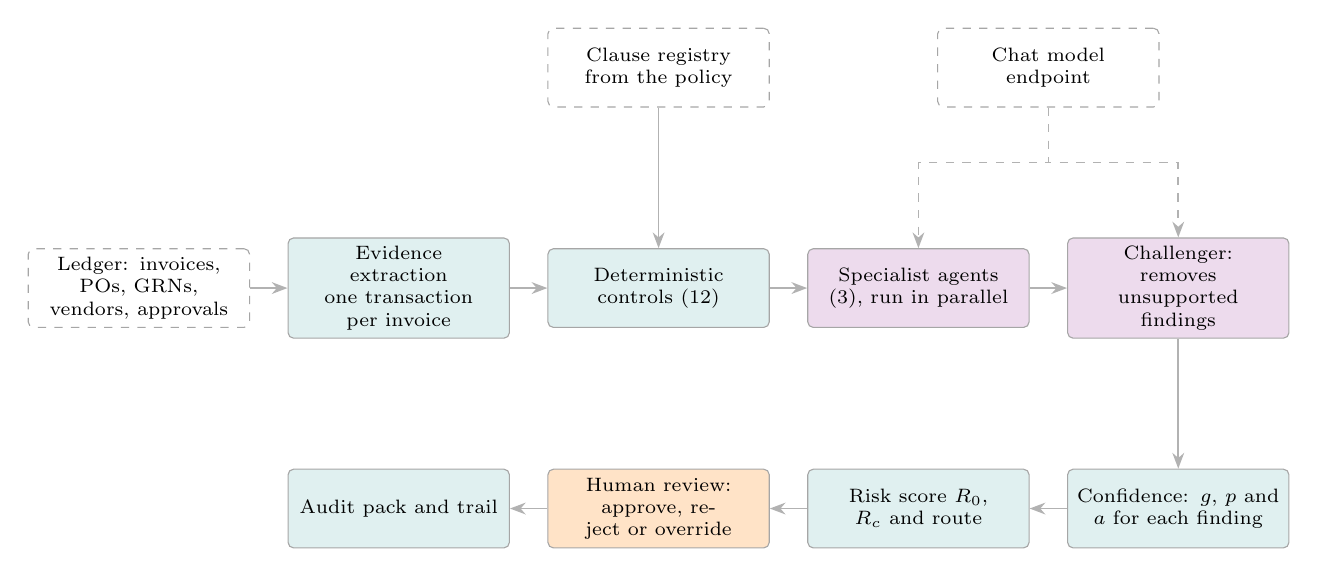
\begin{tikzpicture}[
  box/.style={draw=gray!70, rounded corners=2pt, align=center, font=\scriptsize, text width=2.6cm, inner sep=3pt, minimum height=1.0cm, fill=white},
  code/.style={box, fill=teal!12},
  llm/.style={box, fill=violet!14},
  person/.style={box, fill=orange!22},
  data/.style={box, dashed},
  arr/.style={-{Stealth[length=2mm]}, semithick, gray!60}]
\node[data] (ledger) at (1.45,0) {Ledger: invoices, POs, GRNs, vendors, approvals};
\node[code] (ext) at (4.75,0) {Evidence\\extraction\\one transaction\\per invoice};
\node[code] (ctl) at (8.05,0) {Deterministic controls (12)};
\node[llm] (agt) at (11.35,0) {Specialist agents (3), run in parallel};
\node[llm] (chl) at (14.65,0) {Challenger:\\removes\\unsupported\\findings};
\node[code] (conf) at (14.65,-2.8) {Confidence: $g$, $p$ and $a$ for each finding};
\node[code] (score) at (11.35,-2.8) {Risk score $R_0$, $R_c$ and route};
\node[person] (rev) at (8.05,-2.8) {Human review: approve, reject or override};
\node[code] (pack) at (4.75,-2.8) {Audit pack and trail};
\node[data] (reg) at (8.05,2.8) {Clause registry from the policy};
\node[data] (llmend) at (13.0,2.8) {Chat model endpoint};
\draw[arr] (ledger.east) -- (ext.west);
\draw[arr] (ext.east) -- (ctl.west);
\draw[arr] (ctl.east) -- (agt.west);
\draw[arr] (agt.east) -- (chl.west);
\draw[arr] (chl.south) -- (conf.north);
\draw[arr] (conf.west) -- (score.east);
\draw[arr] (score.west) -- (rev.east);
\draw[arr] (rev.west) -- (pack.east);
\draw[arr] (reg.south) -- (ctl.north);
\draw[arr,dashed] (llmend.south) -- ++(0,-0.7) -| (agt.north);
\draw[arr,dashed] (llmend.south) -- ++(0,-0.7) -| (chl.north);
\end{tikzpicture}
\caption{The audit pipeline for one invoice under configuration C5. Teal: deterministic code; violet: calls a language model; orange: a person; dashed: data or an external service. The clause registry feeds the controls, and the model endpoint serves the agents and the challenger.}
\label{fig:pipeline}
\end{figure}

\begin{table}[htbp]
\caption{The configurations. Each adds stages to the one before it.}
\label{tab:configs}
\centering
\small
\begin{tabular}{L{2.2cm}L{1.5cm}L{4.2cm}L{4.0cm}L{2.2cm}}
\toprule
Configuration & Controls & Language-model agents & Challenger and confidence & Needs a model \\
\midrule
C0 & no & none; isolation forest and one-class SVM, for evaluation only & none & no \\
C1 & yes & none & none & no \\
C2 & no & one prompt over the whole policy & none & yes \\
C3 & yes & three specialist agents & none & yes \\
C4 & yes & three specialist agents & challenger & yes \\
C5 & yes & three specialist agents & challenger; confidence from three re-runs & yes \\
\bottomrule
\end{tabular}
\end{table}

The routing rule means that configuration C1, which has no language-model findings, never samples: its confidences are all 1, so its two scores are equal. The benchmark result for C1 confirms this (Section~\ref{sec:measured}).

\subsection{Policy as data}
The policy document is the input. Its rules become a clause registry: for each of the sixteen rules, a title, a severity, a kind (control or judgement) and its parameter values. The reference policy has fourteen parameter values. Twelve rules are controls, executed by code; four are judgement rules, which go to the agents. A control contains no constant of its own: the tolerance, the daily count, the approval limits and the other values are read from the registry (Table~\ref{tab:rules}).

\begin{table}[htbp]
\caption{The sixteen rules of the reference policy: the twelve controls and the four judgement rules}
\label{tab:rules}
\centering
\small
\begin{tabular}{L{1.4cm}L{5.6cm}L{8.3cm}}
\toprule
Rule & Control, or judgement rule & Wording read from the policy (the value is part of the rule) \\
\midrule
2.1.1 & Amount match & difference of up to 1\% of the purchase-order amount \\
2.1.2 & Quantity match & billed quantity against the quantity received \\
2.1.3 & Missing purchase order or goods receipt & none \\
2.1.4 & \textit{Judgement}: goods-receipt remark contradicts the billed quantity & read by an agent \\
2.1.5 & \textit{Judgement}: description does not match the purchase order & read by an agent \\
2.2.1 & Exact duplicate invoice number & none \\
2.2.2 & \textit{Judgement}: near-duplicate invoice with a re-keyed number & read by an agent \\
3.1.1 & GSTIN format & exactly 15 alphanumeric characters \\
3.1.2 & GSTIN state code & a state code from 01 to 37 \\
3.1.3 & GSTIN against the vendor master & none \\
4.1.1 & Same-day splitting & at most 3 invoices dated on the same day \\
4.1.2 & \textit{Judgement}: purchases split across days to stay below a limit & as a guide, 7 days, within 15\% of the limit; read by an agent \\
4.2.1 & Non-business day & dated on a Saturday or Sunday \\
4.3.1 & Round amount & an exact multiple of INR 10,000 \\
4.4.1 & Blocked vendor & registration status Suspended \\
5.1.1 & Approval limit & the limits of four roles, such as Manager and Senior Manager \\
\bottomrule
\end{tabular}
\end{table}

\begin{figure}[htbp]
\centering
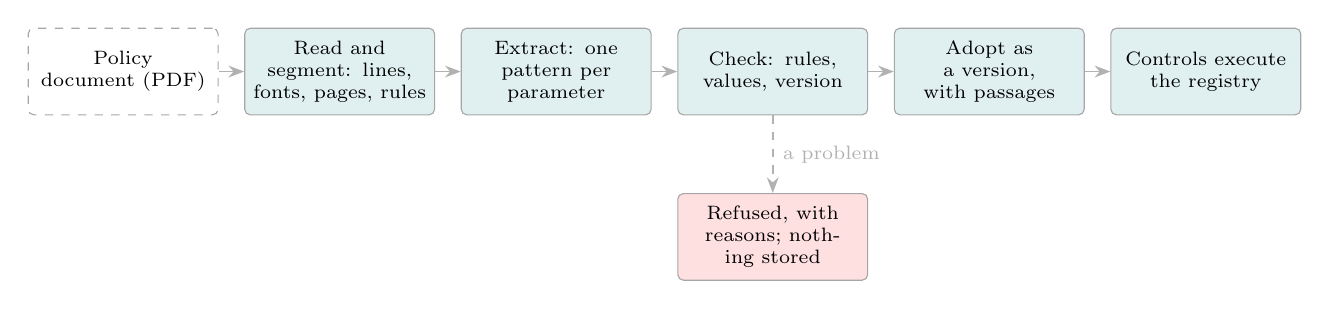
\begin{tikzpicture}[
  box/.style={draw=gray!70, rounded corners=2pt, align=center, font=\scriptsize, text width=2.2cm, inner sep=3pt, minimum height=1.1cm, fill=white},
  code/.style={box, fill=teal!12},
  data/.style={box, dashed},
  bad/.style={box, fill=red!12},
  arr/.style={-{Stealth[length=2mm]}, semithick, gray!60}]
\node[data] (pdf) at (1.1,0) {Policy\\document (PDF)};
\node[code] (read) at (3.85,0) {Read and segment: lines, fonts, pages, rules};
\node[code] (ext) at (6.6,0) {Extract: one pattern per parameter};
\node[code] (chk) at (9.35,0) {Check: rules, values, version};
\node[code] (ado) at (12.1,0) {Adopt as a version, with passages};
\node[code] (ctl) at (14.85,0) {Controls execute the registry};
\node[bad] (ref) at (9.35,-2.1) {Refused, with reasons; nothing stored};
\draw[arr] (pdf.east) -- (read.west);
\draw[arr] (read.east) -- (ext.west);
\draw[arr] (ext.east) -- (chk.west);
\draw[arr] (chk.east) -- (ado.west);
\draw[arr] (ado.east) -- (ctl.west);
\draw[arr,dashed] (chk.south) -- node[midway,right,font=\scriptsize]{a problem} (ref.north);
\end{tikzpicture}
\caption{Policy as data. A document is either adopted as a version, after every rule and value has been checked, or refused with the reasons. The controls then run the adopted registry.}
\label{fig:policyflow}
\end{figure}

\subsection{Data model}
The store has the same tables on SQLite and on PostgreSQL. The column types differ: money is \texttt{NUMERIC(15,2)} on PostgreSQL and \texttt{REAL} on SQLite. Table~\ref{tab:data} lists the groups.

\begin{table}[htbp]
\caption{The tables and views of the store}
\label{tab:data}
\centering
\small
\begin{tabular}{L{2.3cm}L{6.2cm}L{6.8cm}}
\toprule
Group & Tables and views & Holds \\
\midrule
Ledger & \texttt{vendor\_master}, \texttt{purchase\_orders}, \texttt{goods\_receipts}, \texttt{invoices}, \texttt{approval\_logs} & The transactions that are audited: 20,000 invoices in the large ledger. \\
Policy & \texttt{company\_policies}, \texttt{policy\_clauses}, \texttt{policy\_parameters}, \texttt{policy\_documents}, \texttt{policy\_chunks} & Policy versions, the clause registry, the parameter values, the ingested documents and their passages. \\
Audit & \texttt{audit\_runs}, \texttt{audit\_results}, \texttt{audit\_flags}, \texttt{audit\_trail}, \texttt{review\_decisions} & Every run and result, the findings with their evidence, the trail entries and the reviewers' decisions. \\
Other & \texttt{benchmark\_labels}, \texttt{meta} & The labels of the synthetic ledgers, which the pipeline never reads, and facts about the database. \\
Views & \texttt{v\_latest\_results}, \texttt{v\_review\_queue} & The current result of each invoice, and the invoices waiting for a reviewer. \\
\bottomrule
\end{tabular}
\end{table}

\subsection{Services and how they run}
The layers run as the services of Table~\ref{tab:services}. In the experiments all of them ran on one laptop; they are separable, but a deployment on several machines has not been measured.

\begin{table}[htbp]
\caption{The services and the commands that start them}
\label{tab:services}
\centering
\small
\begin{tabular}{L{3.6cm}L{5.6cm}L{6.1cm}}
\toprule
Service & How it runs & Default address and notes \\
\midrule
REST API and web application & \texttt{python -m auditiq serve} & \texttt{http://127.0.0.1:8000}; serves the built frontend and the API description at \texttt{/api/docs} \\
Web application, development & \texttt{npm run dev} in \texttt{frontend/} & \texttt{http://localhost:5173}; reloads on change and forwards \texttt{/api} to port 8000 \\
Streamlit dashboard & \texttt{python -m streamlit run app/dashboard.py} & \texttt{http://localhost:8501}; the simpler interface \\
Command line & \texttt{python -m auditiq} with setup, run, decide, policy, ask, export & The same modules as the API \\
Audit workers & \texttt{python -m auditiq run}; the evaluation runners & Invoices are independent, so several can be audited at once \\
Chat and embedding models & Ollama, or any OpenAI-compatible server & \texttt{http://localhost:11434/v1} in the sample configuration; \texttt{qwen2.5:7b-ctx12k} and \texttt{nomic-embed-text} \\
PostgreSQL 17 (optional) & \texttt{python scripts/pg\_local.py start} for a local server & Port 5544 for the local server; SQLite is the default \\
\bottomrule
\end{tabular}
\end{table}

\clearpage
\subsection{Technology}
\begin{table}[htbp]
\caption{The technology of each part, with the minimum versions set in the project}
\label{tab:tech}
\centering
\small
\begin{tabular}{L{3.6cm}L{12.1cm}}
\toprule
Part & Technology \\
\midrule
Pipeline & LangGraph $\geq$ 1.0 \\
REST API & FastAPI $\geq$ 0.115, Uvicorn $\geq$ 0.34, Pydantic, python-multipart $\geq$ 0.0.18 \\
Store & SQLite (standard library); PostgreSQL 17 with psycopg $\geq$ 3.2 \\
Policy reading and generation & PyMuPDF $\geq$ 1.24 for reading; Python regular expressions; a JSON clause registry; ReportLab $\geq$ 4 for the policy documents of the experiments \\
Analysis and baselines & NumPy $\geq$ 2.0, pandas $\geq$ 2.2, scikit-learn $\geq$ 1.5, statsmodels $\geq$ 0.14; Faker $\geq$ 20 for the synthetic ledgers \\
Models & Ollama with \texttt{qwen2.5:7b} (12,288-token context); \texttt{nomic-embed-text} for policy search; any OpenAI-compatible server \\
Dashboard & Streamlit $\geq$ 1.46 \\
Web application & React 18.3, TypeScript 5.6, Vite 6.4, React Router 7.18, three.js 0.170, React Three Fiber 8.17, drei 9.122 \\
Tests and checks & pytest and ruff (Python); Vitest 4.1, Testing Library, jsdom and ESLint 9.39 (frontend) \\
Continuous integration & GitHub Actions: a Python job on SQLite and on a PostgreSQL 17 service, and a frontend job \\
Paper & LaTeX, IEEEtran; compiled with Tectonic \\
\bottomrule
\end{tabular}
\end{table}

% --------------------------------------------------------- 4 extra features
\section{Extra features}
\label{sec:features}
The base system is the multi-agent pipeline. The features below are what this project adds to it. F1 is the feature the paper is about. F2 to F9 are the features built around it, so that it can be used, measured and reviewed. Each description gives what the feature does, its input and output, its logic, its technology, and its status and evidence.

\subsection{F1 Policy-driven deterministic controls}
\textbf{What it does.} The policy document is the configuration of the audit. The controls that can be decided by comparing fields take every threshold from the adopted policy version, and no control keeps a value of its own.

\textbf{Input and output.} The input is a policy PDF in the template wording, and the ledger. The output is a clause registry (sixteen rules, fourteen parameter values), with the passage and page each rule came from; and, for each invoice, a list of findings, each with its rule, severity, evidence and citation.

\textbf{Logic.} Six steps. (1) Every text line is read with its font size, position and page. (2) The rules are found by layout: the body size is the most frequent font size, a heading is at least one point larger, and a line beginning ``Rule $n.n$ (severity),'' opens a rule. (3) Each threshold is extracted with one pattern matched in the wording of its rule; the approval limits come from the table of roles. (4) The document is checked, and refused if needed: a rule the system executes is absent, a threshold is not found in its rule, a rule has no control, a value is not meaningful, or no version is stated. A refused document stores nothing, and the reasons are given. (5) The document is adopted as a new version. (6) Each control runs on the transaction with the registry's values, using integer paise, so that rounding cannot move a decision at a boundary.

\textbf{Technology.} PyMuPDF for reading; Python regular expressions for extraction; a JSON clause registry; Python controls without a library; SQLite or PostgreSQL for storage.

\textbf{Status and evidence.} Built and measured (Section~\ref{sec:measured}). Across fourteen policy documents, 196 of 196 values and 224 of 224 rules were read correctly, in less than a tenth of a second per document. Across 560,000 audits, the policy-driven controls made no wrong decision; on 20 held-out random documents, none in 800,000. A robustness test with 16 edited documents found two ambiguous documents that were adopted; the reader now refuses both.

\textbf{Limits.} The pattern reading accepts the template wording only. A rule with new semantics needs a new control. The ground truth of the rule-defined classes implements the same written rules, so perfect scores there check the implementation, not the rules.

\subsection{F2 Policy adoption and change without code}
\textbf{What it does.} An auditor uploads a new policy document, sees which thresholds would change, adopts the document, and re-audits the ledger under the active version. No file of the system is edited.

\textbf{Input and output.} The input is the PDF, and the choice to activate the version and to replace a stored version of the same number. The output is a new stored version with its passages; a preview that lists each changed value (rule, parameter, active value and new value), or the reasons the document was refused; and the re-audit results.

\textbf{Logic.} The preview reads the document and compares it with the active version. The upload is limited to 20\,MB and must start with the PDF signature. Adoption stores the version; activation makes it the one the next audit applies. A re-audit adds a result for each invoice and keeps the earlier ones, so an invoice keeps its history under the policies that applied to it.

\textbf{Technology.} The REST endpoints for preview, adoption and activation; the background job with progress for the re-audit; the command \texttt{policy adopt}; the Policy page of the web application.

\textbf{Status and evidence.} Built and measured on the ledger of 20,000 invoices. Reading and storing the strict policy document took 0.03 seconds, and re-auditing the ledger took 43 seconds (50 before the change; \texttt{results/application\_demo.md}). Findings went from 300 to 6,546, invoices waiting for review from 240 to 6,353, and invoices approved automatically from 19,760 to 13,647.

\subsection{F3 Policies written in their own wording}
\textbf{What it does.} When a document is not in the template wording, a language model reads it and proposes the rules and the thresholds. Code checks each proposal against the document. A named person confirms what is adopted.

\textbf{Input and output.} The input is any policy PDF and a chat model. The output is, for each rule, its passage and page; for each value, the proposed value, the words quoted from the document, and a status: verified, or held back with the reason. After confirmation, a new policy version.

\textbf{Logic.} The model must return, for each rule and value, the words it was taken from. Code accepts a quote only if it occurs in the document word for word. It accepts a value only if the value is written in the quote of its own rule, as digits, in Indian digit grouping, or as a number word from two to twenty. Anything else is held back. The reviewer compares each verified value with its quote, supplies the held-back values and any missing passage, enters a name, and adopts.

\textbf{Technology.} A local 7B model (Qwen2.5, 12,288-token context, temperature 0) behind an OpenAI-compatible endpoint; Python verification; the review step in the command line (\texttt{policy adopt --llm}) and in the web application.

\textbf{Status and evidence.} Built and measured on six documents in two styles (three memoranda and three handbooks), each stating three policies: 84 values in all (Table~\ref{tab:freeform}). The model proposed 80 of 84 values correctly and located 92 of 96 rules. After confirmation, four of the six documents give exactly the intended policy.

\textbf{Limits.} The two values that the check passed are the same error in both handbooks: the status ``Blacklisted'' was added to the blocked statuses, and the word occurs in the quoted passage, so the check cannot see it. The confirming person is the safeguard. The check has not been tuned on this case, to avoid tuning on the evaluation set.

\subsection{F4 Controls first, then specialist agents, challenger and confidence}
\textbf{What it does.} The controls decide what can be decided by comparing fields. The language models judge only the four judgement rules: a goods-receipt remark that contradicts the billed quantity (2.1.4), a description that does not match the purchase order (2.1.5), a near-duplicate invoice with a re-keyed number (2.2.2), and purchases split across days to stay below a limit (4.1.2). A challenger removes unsupported agent findings. The confidence of each agent finding measures how stable it is.

\textbf{Input and output.} The input is the transaction, the control findings and the policy text the agents need. Each agent sees the records of its own remit and, for the vendor, at most 40 of its other invoices. The output is the agent findings with their evidence, the findings the challenger removed with the reason, a confidence for each finding, and a route.

\textbf{Logic.} The rules of the pipeline are described in Section~\ref{sec:arch}: the agents run in parallel, code discards findings outside their remit, the challenger may only remove, and in C5 each finding is re-run three times at temperature 0.7 to measure agreement. The route is set by the two scores: escalation when the confidence-weighted score reaches 50, sampled review when only the count-based score does, and approval otherwise.

\textbf{Technology.} LangGraph graphs for the configurations C1 to C5; an OpenAI-compatible client with a response cache, retries and token accounting.

\textbf{Status and evidence.} Built and tested with a scripted model, and run on a pilot of 20 invoices with the local 7B model (Section~\ref{sec:pilot}). It has not been run on the benchmark.

\textbf{Limits.} Confidence measures stability, not correctness. In the pilot, two wrong findings on hard negatives had confidence 0.67 and 1.00. The accuracy of the agents on the judgement rules is not measured at benchmark scale.

\subsection{F5 Forensic trail and review workflow}
\textbf{What it does.} Every audit stores the result, the findings with their evidence, the findings the challenger removed and why, one trail entry per stage, and the policy version that was applied. A reviewer then approves, rejects or overrides the invoice. An override needs a written justification.

\textbf{Input and output.} The input is the result, the reviewer's name, the decision and the justification. The output is an audit pack and a trail that together show how each decision was reached, and the review queue of invoices waiting for a decision.

\textbf{Logic.} A result is \texttt{AUTO\_APPROVED}, \texttt{PENDING\_REVIEW} or \texttt{NOT\_SAMPLED}. A decision moves a pending result to \texttt{REVIEW\_APPROVED}, \texttt{REVIEW\_REJECTED} or \texttt{REVIEW\_OVERRIDDEN}, and is recorded as the last trail entry. A new audit of the same invoice adds a result rather than replacing the old one, and the newer result takes its place in the queue.

\textbf{Technology.} Relational tables and two views, on both backends.

\textbf{Status and evidence.} Built and tested on both backends. The invoice page of the web application shows the pack, the trail with the tokens and time of each model call, and the decision form.

\subsection{F6 Copilot with cited answers and checked data queries}
\textbf{What it does.} The copilot answers questions about the policy and about one audited invoice, with citations. It answers questions about the data with one query, which is checked before it runs.

\textbf{Input and output.} The input is a question, optionally with an invoice identifier. The output is an answer with the cited passages (document and page). For a data question, the output is the query and its rows.

\textbf{Logic.} Policy questions retrieve passages by lexical, dense or hybrid ranking, optionally after the question is rewritten. For an audited invoice, the passages of the rules its findings cite come first, and the instructions make the audit record the authority. Data questions: the model writes one \texttt{SELECT}. The code checks that it is a single \texttt{SELECT}, that it names only tables on an allow-list, and runs it on a read-only connection with a row limit and a time limit. On PostgreSQL it runs as the role \texttt{auditiq\_reader}.

\textbf{Technology.} Hybrid retrieval over the policy passages, with the embedding model nomic-embed-text; the chat model for the answers; the query check in Python.

\textbf{Status and evidence.} Retrieval was measured on 48 fixed questions: 16 in the policy's own wording and 32 paraphrases. The lexical ranking finds every question in the policy's wording at rank 1. On the held-out paraphrases, hybrid ranking with question rewriting finds the right passage at rank 1 for 0.625 of the questions and within the top three for 0.938 (16 questions). In a real check, the first answer named the wrong rule, because retrieval by the question's wording ranked the duplicate-invoice rules first. Placing the passages of the cited rules first corrected the answer.

\subsection{F7 REST API with background jobs}
\textbf{What it does.} The REST API exposes the ledger, the review, the policy, the copilot and the measured results over HTTP. It has 22 endpoints (Appendix~\ref{app:api}), and its description is served at \texttt{/api/docs}.

\textbf{Input and output.} The requests are JSON, validated and length-limited, except for the policy upload, which is multipart. The responses are JSON; errors carry a message in \texttt{detail}.

\textbf{Logic.} Every request opens its own database connection, so the API holds no state between requests. Work that takes long runs as a background job on a thread: the request answers with status 202 and a job identifier, and the client polls the job for its progress and its result. The last 200 jobs are kept in memory. A bearer token, when configured, protects every endpoint except the health check, and it is compared in constant time. An unreachable database answers 503 with the reason.

\textbf{Technology.} FastAPI and Uvicorn, with Pydantic for the request models and python-multipart for uploads.

\textbf{Status and evidence.} Built and tested: ten API test functions. Nine of them run on both SQLite and PostgreSQL; the tenth checks the answer when the database cannot be reached.

\subsection{F8 Web application with three-dimensional views}
\textbf{What it does.} The web application is the browser interface for reviewers. It has seven pages: Overview, Review queue, Invoices (search and detail), Policy, Copilot, Pipeline and Results.

\textbf{The three-dimensional views.} (a) The \emph{risk constellation} on the Overview draws every vendor as a sphere. The sector is the vendor's spending category; the height is the highest risk among its invoices; the size grows with its number of invoices; pulsing spheres have invoices waiting for review; violet spheres are blacklisted. Clicking a vendor opens its invoices. (b) The \emph{pipeline graph} shows the stages of the audit; choosing a configuration lights the stages it runs. (c) The \emph{policy-change bars} on the Results page show, for each policy, the share of invoices that a frozen system decides against the policy in force. Each view has a table with the same data beside it, and a message when the browser has no WebGL.

\textbf{Technology.} React 18 with TypeScript, Vite, React Router 7, three.js~\cite{threejs} and React Three Fiber~\cite{r3f} with drei. The constellation draws all vendors as one instanced mesh, with one colour per vendor.

\textbf{Status and evidence.} Built and tested: 28 frontend tests, including the three 3D scenes, rendered with React Three Fiber's test renderer. Lint, type checking, the production build and the dependency audit are clean. All seven pages were checked in a browser. The 3D library is in its own bundle of about 822\,kB (221\,kB gzipped), which loads only with the Overview, Pipeline and Results pages.

\subsection{F9 Two storage backends and bulk processing}
\textbf{What it does.} The same schema runs on SQLite, a single file that is the default, and on PostgreSQL 17, a server for several users. Money is \texttt{NUMERIC} on PostgreSQL and \texttt{REAL} on SQLite; the application sees floats and ISO dates either way.

\textbf{Logic.} Batch runs read the ledger in bulk, 200 invoices at a time. A connection to an up-to-date database reads a schema stamp and changes nothing. On PostgreSQL, creating a new schema holds an advisory lock. Before this was fixed, every connection re-created the views, and concurrent web requests could deadlock.

\textbf{Status and evidence.} Measured: a batch audit of 20,000 invoices under C1 on PostgreSQL took 2 minutes 58 seconds after bulk extraction, against 4 minutes 57 seconds before. A test opens 32 connections at once to guard against the deadlock.

% ---------------------------------------------------------- 5 measured
\subsection{F10 Loading a ledger from Excel or a zip archive}
\textbf{What it does.} An organisation brings its own ledger: an Excel workbook with one sheet per table (vendors, purchase orders, goods receipts, invoices, approval log), a \texttt{.zip} archive of the same tables as CSV files, or a folder of them. It is loaded from the Overview page of the web application or of the dashboard, or with \texttt{python -m auditiq ledger import}.

\textbf{Logic.} The ledger is checked before anything is replaced: every table and column is present, every identifier is filled and unique, amounts and dates can be read, and every reference the store enforces points to a record of the ledger. A ledger with any problem is refused with the list of problems. An invoice may name a purchase order that does not exist; that is the exception of rule 2.1.3, not a defect of the file. Spreadsheet cells (dates, numbers, true or false) are read as the text a CSV file would hold. Loading replaces the previous ledger with its results, so the application asks for confirmation, and then offers to audit the new ledger with the controls.

\textbf{Status and evidence.} Built and tested: all six datasets pass the checks; a workbook and a zip archive give exactly the CSV ledger; a workbook typed by hand, with real dates and numbers, is audited with exactly the same findings as the CSV ledger; defective ledgers are refused with their reasons and nothing is replaced. Checked in the browser: a 40-invoice ledger uploaded, loaded and audited.

\section{Measured results}
\label{sec:measured}
Each table below is read from the files that the scripts write under \texttt{results/}, named in its caption. Intervals are 95\% bootstrap intervals over invoices, with 1,000 resamples, where they are shown. Every result is also in \texttt{RESULTS.md} and, machine-readable for programs and other language models, in \texttt{auditiq/\allowbreak results/\allowbreak results.json}. The full report, with the methodology, every result in detail, a per-invoice analysis of the model runs and the threats to validity, is \texttt{REPORT.md} at the root of the repository.

\subsection{Detection against classical detectors}
\begin{table}[htbp]
\caption{Measured. Benchmark: the mean of three ledgers of 5,000 invoices, 8.4\% anomalous. Large ledger: 20,000 invoices, 2.1\% anomalous. Source: \texttt{results/summary.md} and \texttt{evaluation/run\_all.py}.}
\label{tab:detect}
\centering
\small
\begin{tabular}{L{3.2cm}R{2.1cm}R{2.1cm}R{2.1cm}R{2.1cm}R{2.1cm}}
\toprule
System & Recall & Precision & F1 & False positives, ordinary & False positives, hard negatives \\
\midrule
Isolation forest~\cite{liu2008} & 0.577 & 0.501 & 0.536 & 0.044 & 0.403 \\
One-class SVM~\cite{scholkopf2001} & 0.464 & 0.543 & 0.498 & 0.025 & 0.481 \\
Controls (C1) & \textbf{0.714} & \textbf{1.000} & \textbf{0.833} & \textbf{0.000} & \textbf{0.000} \\
\bottomrule
\end{tabular}
\end{table}

On the large ledger, the F1 is 0.211 for the isolation forest, 0.429 for the one-class SVM and 0.833 for the controls. The two detectors are implemented with scikit-learn~\cite{pedregosa2011}, and they choose their thresholds by five-fold cross-fitting, so no invoice is decided with a threshold tuned on its own label. McNemar's exact test, Holm-adjusted, favours the controls over each detector on every benchmark ledger, with adjusted $p$ below $10^{-50}$.

The controls report all ten rule-defined classes and none of the four judgement classes, and they raise no finding on a clean invoice. The one-class SVM reports only about 3\% of the invoices with a malformed or mismatched GSTIN or a missing reference (classes R4, R5 and R8). Both detectors report every near-duplicate (class J1), whose copied amount and vendor make it unusual for a statistical method. Of the judgement classes J2 to J4, the detectors report at most 22\%, and the controls none, by design.

\subsection{Policy change}
\begin{table}[htbp]
\caption{Measured. Fourteen policy documents, each applied to 40,000 invoices of five ledgers, against a system whose thresholds are frozen at version 2.5. The policy-driven controls had adherence 1.000 under every document. Source: \texttt{results/policy\_change.md}.}
\label{tab:policy}
\centering
\small
\begin{tabular}{L{4.2cm}R{2.5cm}R{2.5cm}R{2.5cm}R{2.5cm}}
\toprule
Policy in force & Decisions moved & Frozen adherence & Missed escalations & Unsupported findings \\
\midrule
Strict policy & 12,274 & 0.693 & 12,012 & 0 \\
Manager limit 50,000 & 7,677 & 0.808 & 7,514 & 0 \\
Senior Manager limit 250,000 & 4,259 & 0.894 & 4,161 & 0 \\
Lenient policy & 380 & 0.991 & 0 & 380 \\
Version 2.6 & 302 & 0.992 & 0 & 302 \\
\bottomrule
\end{tabular}
\end{table}

A tightening leaves a frozen system silent: it approves invoices that the policy in force sends to review. A loosening costs reviewer time: it raises findings that the policy no longer supports. The policy-driven controls read each document in less than a tenth of a second, and they audited the 560,000 invoice decisions in 14 seconds.

\subsection{Every ledger through the deployed system}
Each of the six ledgers was written as an Excel workbook, loaded from it through the checked import, and audited with the controls through the data store; the outcome was read back from the store. Source: \texttt{results/\allowbreak ledger\_runs.md}.

\begin{table}[htbp]
\caption{Measured. Every ledger loaded from a workbook and audited with the controls (C1) under version 2.5, through the store.}
\label{tab:ledgerruns}
\centering
\small
\begin{tabular}{L{4.0cm}rrrr}
\toprule
Ledger & Invoices & Findings & Escalated & Approved \\
\midrule
bench\_seed\_101 & 5,000 & 300 & 240 & 4,760 \\
bench\_seed\_202 & 5,000 & 300 & 240 & 4,760 \\
bench\_seed\_303 & 5,000 & 300 & 240 & 4,760 \\
large\_seed\_505 & 20,000 & 300 & 240 & 19,760 \\
pilot\_seed\_909 & 5,000 & 300 & 240 & 4,760 \\
swap\_seed\_404 & 5,000 & 150 & 150 & 4,850 \\
\bottomrule
\end{tabular}
\end{table}

On each benchmark ledger every one of the 300 rule-defined anomalies got a finding; 240 were escalated (90 critical, 150 high), and the other 60, with only low or medium findings, were approved with the finding recorded. No hard negative and no ordinary invoice got a finding; the judgement anomalies are left to the agents.

\subsection{Held-out policy documents}
Twenty further policy documents were drawn at random (seed 2026) from values that played no part in building or checking the reader; each changes one to five values. Source: \texttt{results/\allowbreak policy\_heldout.md}. The system read 280 of 280 values and 320 of 320 rules correctly, adopted all twenty documents, and the policy-driven controls made no wrong decision in 800,000 invoice audits. A frozen system decided up to 7,953 invoices (19.9\%) against the policy in force. This measures what the paper had listed as the expected value X1.

\subsection{Robustness of the reader}
The reference policy was edited in sixteen ways and each edited PDF was read. Source: \texttt{results/\allowbreak policy\_robustness.md}. All seven edits that keep every value (extra prose, reordered rules, long rules, page breaks, a reordered table, a changed severity, Indian digit grouping) were read correctly; all seven defects (a threshold or rule removed, an unknown rule, no version, a day that is not a weekday, no approval table, a threshold in words) were refused with the reason. The two ambiguous documents (a rule stated twice with two values, an approval table without one role) were adopted in the first run; both checks were added to the reader, with tests, and both are now refused: 16 of 16 as required.

\subsection{Scalability of the control stage}
\begin{table}[htbp]
\caption{Measured. Throughput of the control stage for 300,000 invoice audits on a laptop with 12 logical CPUs; every run found the same 16,840 findings. Source: \texttt{results/scalability.md}.}
\label{tab:scal}
\centering
\small
\begin{tabular}{rrrr}
\toprule
Worker processes & Seconds & Invoices per second & Speed-up \\
\midrule
1 & 5.29 & 56,660 & 1.00 \\
2 & 3.10 & 96,724 & 1.71 \\
4 & 2.50 & 119,780 & 2.12 \\
8 & 1.74 & 172,226 & 3.04 \\
\bottomrule
\end{tabular}
\end{table}

The cost per invoice does not grow with the ledger: it was 17.8, 19.4 and 18.3 $\mu$s at 5,000, 20,000 and 40,000 invoices. The speed-up is below the number of processes because the processor has two performance cores and eight slower efficiency cores.

\subsection{Policies written in their own wording}
\begin{table}[htbp]
\caption{Measured. Six policy documents, 14 values and 16 rules each, read by a local 7B model and checked by code. Source: \texttt{results/policy\_llm.md}.}
\label{tab:freeform}
\centering
\small
\begin{tabular}{L{6.2cm}rrr}
\toprule
 & Memoranda & Handbooks & All \\
\midrule
Values & 42 & 42 & 84 \\
Right, verified by the code check & 28 & 28 & 56 \\
Right, held back for the reviewer & 12 & 12 & 24 \\
Wrong, caught by the check & 2 & 0 & 2 \\
Wrong, passed the check & 0 & 2 & 2 \\
Rules located & 47 of 48 & 45 of 48 & 92 of 96 \\
\bottomrule
\end{tabular}
\end{table}

The held-back values are all approval limits whose quote did not contain the amount, or was not found in the document. The reviewer supplies them. Each document took 282 to 393 seconds to read on the laptop.

\subsection{Pilot of the language-model stages (20 invoices)}
\label{sec:pilot}
The language-model stages were run with the same local model on 20 invoices of a development ledger, which no reported benchmark uses: one invoice of each of the fourteen anomaly classes, one of each of the five hard-negative types, and one ordinary invoice. \emph{Twenty invoices are a pilot.} The intervals are wide (for example, the recall of C3 is 0.929 with a 95\% interval from 0.750 to 1.000), and no difference between the configurations is significant: C3 against C2 gives a Holm-adjusted $p$ of 0.196. The pilot shows that every stage runs against a real model and what an invoice costs. It does not estimate how well a model audits.

\begin{table}[htbp]
\caption{Measured pilot: 20 invoices, a local 7B model on a laptop CPU. Not a benchmark result. Source: \texttt{results/pilot\_seed\_909/pilot20.md}.}
\label{tab:pilot}
\centering
\small
\begin{tabular}{L{6.0cm}rrrrr}
\toprule
Measure & C1 & C2 & C3 & C4 & C5 \\
\midrule
Invoice-level recall & 0.714 & 0.929 & 0.929 & 0.857 & 0.857 \\
Invoice-level precision & 1.000 & 0.722 & 0.812 & 0.800 & 0.800 \\
Macro-F1, rule-defined classes & 1.000 & 0.095 & 1.000 & 1.000 & 1.000 \\
Judgement classes found (of 4) & 0 & 1 & 2 & 1 & 1 \\
Hard negatives flagged (of 5) & 0 & 4 & 3 & 3 & 3 \\
Ordinary invoice flagged (of 1) & 0 & 1 & 0 & 0 & 0 \\
Model findings naming a violated rule & -- & 0.067 & 0.111 & 0.111 & 0.111 \\
Invoices sent to sampled review & 0 & 0 & 0 & 0 & 2 \\
Model calls per invoice & 0 & 1.15 & 3.00 & 3.60 & 4.95 \\
Tokens per invoice & 0 & 5,835 & 9,557 & 12,005 & 16,779 \\
\bottomrule
\end{tabular}
\end{table}

The pilot shows four things, and only these. The controls first decide the rule-defined classes exactly. A single prompt over the whole policy (C2) flagged 18 of the 20 invoices, and only 5 of its 75 findings named a rule that the invoice violates. The agents in C3 found the goods-receipt remark and the near-duplicate, missed the structuring across days, and cited the wrong rule for the description mismatch. The challenger in C4 removed nine agent findings, one of them right. Confidence in C5 sent two invoices to sampled review, both true anomalies. The wrong findings on the hard negatives kept their confidence, which again shows that confidence measures stability rather than correctness.

\subsection{The language-model stages on a benchmark sample (34 invoices)}
\label{sec:sample}
All five configurations were run with the frozen prompts on 34 invoices of benchmark ledger 101, which no prompt was ever tried on: five of each judgement class, two of each hard-negative type and four ordinary invoices, drawn with a fixed seed. Source: \texttt{results/bench\_seed\_101/sample34.md}. No difference between configurations is significant on 34 invoices (C3 against C2: Holm-adjusted $p$ = 0.277).

\begin{table}[htbp]
\caption{Measured on a sample: 34 invoices of benchmark ledger 101, local 7B model. Source: \texttt{results/bench\_seed\_101/sample34.md}.}
\label{tab:sample}
\centering
\small
\begin{tabular}{L{6.0cm}rrrrr}
\toprule
Measure & C1 & C2 & C3 & C4 & C5 \\
\midrule
Judgement anomalies found (of 20) & 0 & 4 & 12 & 8 & 8 \\
Hard negatives flagged (of 10) & 0 & 7 & 8 & 4 & 4 \\
Ordinary invoices flagged (of 4) & 0 & 4 & 3 & 2 & 2 \\
Model findings naming a violated rule & -- & 0.031 & 0.375 & 0.471 & 0.471 \\
Invoices sent to sampled review & 0 & 0 & 0 & 0 & 4 \\
Failed stages & 0 & 4 & 0 & 0 & 0 \\
Model calls per invoice & 0 & 1.21 & 3.00 & 3.74 & 5.24 \\
Tokens per invoice & 0 & 6,259 & 9,678 & 12,562 & 17,828 \\
\bottomrule
\end{tabular}
\end{table}

The agents (C3) found 12 of the 20 judgement anomalies: all five near-duplicates, four of five goods-receipt remarks, two of five cases of structuring and one of five description mismatches; 12 of their 32 findings named a violated rule. The challenger (C4) halved the false alarms on hard negatives but removed four of the five correct near-duplicate findings. Confidence (C5) sent four invoices to sampled review, three of them true anomalies. The single prompt (C2) flagged almost every invoice and only 4 of its 128 findings named a violated rule. With a 7B model the agents stay below the expected values X2 and X3 of the paper.

\subsection{Quality checks}
Table~\ref{tab:quality} lists the checks run on the code and the results, and the end-to-end reproduction of the datasets and experiments.

\begin{table}[H]
\caption{The checks run on the code and the results of each on 18 October 2026}
\label{tab:quality}
\centering
\small
\begin{tabular}{L{4.2cm}L{11.5cm}}
\toprule
Check & Result \\
\midrule
Python tests & 330 test cases collected. 327 pass and 3 are skipped on the development laptop. One of the skipped tests is skipped on PostgreSQL by design, so it is also skipped in continuous integration. \\
Frontend tests & 28 pass (Vitest, Testing Library, and the three 3D scenes). \\
API tests & 10 test functions: nine run on SQLite and on PostgreSQL, and one checks the answer when the database is unreachable. \\
Lint and types & ruff is clean for the Python code; ESLint and the TypeScript check are clean for the frontend. \\
Dependencies and build & \texttt{npm audit} reports no known vulnerability; the production build succeeds. \\
Continuous integration & The Python job and the frontend job both succeed on every push to \texttt{main}. \\
End-to-end check & All six datasets regenerated: 54 of 54 files identical byte for byte. Every experiment without a model re-run on 18 October 2026: every count, value and decision identical; only the timings differ. The policy reading by the model and the retrieval experiment, re-run from the cached model replies: identical. \\
\bottomrule
\end{tabular}
\end{table}

% ------------------------------------------------------ 6 limitations
\section{Limitations and what is not measured}
\begin{itemize}
\item \textbf{The language-model configurations C2 to C5 are measured only on samples} of 20 and 34 invoices. The development laptop has no GPU; a 7B model needs minutes per call there, and a benchmark ledger needs about 1,200 invoices with several calls each. The expected values in the paper for these stages are targets fixed before measurement. They are not results.
\item \textbf{The controls and their ground truth implement the same written rules.} Perfect scores on the rule-defined classes verify the implementation. They do not show that the rules catch real fraud.
\item \textbf{The judgement classes J2 to J4} are not found by the controls by design, and the agents were measured on them only in the two samples.
\item \textbf{The ledgers are synthetic}, generated by the project. The counts describe how these ledgers react to these changes, not the books of an organisation.
\item \textbf{Pattern reading accepts only the template wording.} The model-assisted path was measured on six short documents written by the authors, with one 7B model. Two wrong values passed its check, so the confirming person remains a required safeguard.
\item \textbf{Confidence measures stability, not correctness.}
\item \textbf{The web application has one shared token and no user accounts.} The reviewer's name is typed, not authenticated. Background jobs live in the memory of one process; a restart forgets them, although the work they did is in the database.
\item \textbf{Everything ran on one laptop.} The services are separable, but their behaviour on several machines has not been measured.
\end{itemize}

% -------------------------------------------------------------- 7 next steps
\section{Next steps}
\begin{enumerate}
\item \textbf{The benchmark runs.} Obtain a faster model endpoint, then run configurations C2 to C5 on the three benchmark ledgers, with the same reports and the same paired tests. The expected values of the paper are the targets. Each benchmark ledger needs, by an estimate from the prompt sizes (not a measurement), about 12 million prompt tokens for C2 to C4.
\item \textbf{Decide the class of J1.} Make near-duplicate invoices a rule-defined class with a control for rule 2.2.2 (recommended), or keep them as a judgement class.
\item \textbf{Rotate the old database password} found in the reference folder. This is an action for the owner of the old database.
\item \textbf{Confirm the details of the third author} and choose the template and page limit of the target venue.
\item \textbf{Before any multi-user deployment:} user accounts and roles for the web application, and a job queue in place of the in-memory jobs.
\end{enumerate}

% ---------------------------------------------------------------- appendices
\appendix
\section{REST API endpoints}
\label{app:api}
\begin{table}[htbp]
\caption{The 22 endpoints of the REST API. Endpoints marked as jobs answer with status 202 and a job identifier.}
\label{tab:api}
\centering
\small
\begin{tabular}{L{6.4cm}L{9.3cm}}
\toprule
Method and path & Purpose \\
\midrule
\texttt{GET /api/health} & Version, backend, ledger, active policy and model; no token needed \\
\texttt{GET /api/overview} & Counts by state, route and risk; findings by rule; recent runs; vendors with invoices waiting \\
\texttt{GET /api/risk-map} & Every vendor, for the three-dimensional constellation \\
\texttt{GET /api/pipeline} & The stages and the stages of each configuration; no token needed \\
\texttt{GET /api/queue} & Invoices waiting for a reviewer, highest weighted risk first \\
\texttt{GET /api/invoices} & Search invoices by identifier or vendor name \\
\texttt{GET /api/invoices/\{id\}} & The records, the vendor history, the latest result with its pack and trail \\
\texttt{POST /api/results/\{id\}/decision} & Record a decision: approve, reject or override \\
\texttt{POST /api/invoices/\{id\}/audit} & Audit one invoice under a configuration (job) \\
\texttt{GET /api/policy} & Versions, the rules of the active version, the ingested documents \\
\texttt{POST /api/policy/activate} & Make a stored version the active one \\
\texttt{POST /api/policy/preview} & Upload a policy PDF; the thresholds and the changes \\
\texttt{POST /api/policy/adopt} & Adopt a previewed document \\
\texttt{POST /api/policy/propose} & A model reads a document in its own wording (job) \\
\texttt{POST /api/policy/confirm} & Adopt a proposal after the reviewer's confirmation \\
\texttt{POST /api/policy/apply} & Re-audit the ledger under the active version (job) \\
\texttt{POST /api/ledger} & Upload a ledger (workbook or zip archive); checked, then loaded (job) \\
\texttt{GET /api/search} & Search the policy documents \\
\texttt{POST /api/copilot/ask} & A policy or invoice question, with citations (job) \\
\texttt{POST /api/copilot/data} & A question about the data, answered by one checked query (job) \\
\texttt{GET /api/jobs/\{id\}} & The state and the result of a job \\
\texttt{GET /api/results} & The measured results, as the scripts wrote them \\
\bottomrule
\end{tabular}
\end{table}

\section{Repository layout}
\begin{table}[htbp]
\caption{The main folders of the repository}
\label{tab:layout}
\centering
\small
\begin{tabular}{L{4.5cm}L{11.2cm}}
\toprule
Folder & Content \\
\midrule
\texttt{auditiq/} & The pipeline, the database, the policy documents, the copilot, the command line and the REST API (\texttt{api.py}). \\
\texttt{auditiq/frontend/} & The web application: React, TypeScript and React Three Fiber. \\
\texttt{auditiq/auditiq\_bench/} & The dataset generator and its validator. \\
\texttt{auditiq/evaluation/} & Baselines, runners, metrics, statistics and reports. \\
\texttt{auditiq/app/} & The Streamlit dashboard. \\
\texttt{auditiq/policy/} & The clause registry, the templates, the generated policy documents and the free-form documents. \\
\texttt{auditiq/data/}, \texttt{results/}, \texttt{exports/} & The datasets; the measured results; a CSV snapshot of the database. \\
\texttt{auditiq/docs/} & Architecture, operations, the web application, the feature, the datasets and the data dictionary. \\
\texttt{auditiq/tests/} & The Python test suite. \\
\texttt{paper/} & The paper (\texttt{.tex} and \texttt{.pdf}) and the policy section. \\
\texttt{.github/workflows/ci.yml} & Continuous integration. \\
\bottomrule
\end{tabular}
\end{table}

\section{Commands}
To set up the system and run it, from the project folder:
\begin{verbatim}
pip install -e ".[dev]"
python -m auditiq setup --dataset data/large_seed_505
python -m auditiq run --config C1
cd frontend && npm ci && npm run build && cd ..
python -m auditiq serve
\end{verbatim}
The web application is then at \url{http://127.0.0.1:8000}, and the API description at \url{http://127.0.0.1:8000/api/docs}. A ledger of the organisation's own, an Excel workbook or a \texttt{.zip} archive of the CSV files, replaces the sample one on the Overview page, or with
\begin{verbatim}
python -m auditiq ledger import ledger.xlsx
\end{verbatim}
The documents in \texttt{auditiq/docs}, namely \texttt{WEB.md}, \texttt{OPERATIONS.md} and \texttt{ARCHITECTURE.md}, give the details.

% ---------------------------------------------------------------- references
\section*{References}
\addcontentsline{toc}{section}{References}
\sloppy
\begin{thebibliography}{10}
\bibitem{wang2025auditbench} R. Wang, J. Liu, W. Zhao, S. Li, and D. Zhang, ``AuditBench: A benchmark for large language models in financial statement auditing,'' in \textit{AI for Research and Scalable, Efficient Systems} (Communications in Computer and Information Science). Singapore: Springer, 2025, pp. 59--81. [Online]. Available: \url{https://doi.org/10.1007/978-981-96-8912-5_3}
\bibitem{liu2026survey} Q. Liu, L. Yao, Z. Wang, Y. Yang, Y. Tang, D. Cheng, and C. Jiang, ``Large language model-based multi-agent systems for financial markets simulation: A survey,'' \textit{Sci. China Inf. Sci.}, vol. 69, no. 7, Art. no. 171201, 2026. [Online]. Available: \url{https://doi.org/10.1007/s11432-026-4986-x}
\bibitem{liu2008} F. T. Liu, K. M. Ting, and Z.-H. Zhou, ``Isolation forest,'' in \textit{Proc. 8th IEEE Int. Conf. Data Mining (ICDM)}, 2008, pp. 413--422. [Online]. Available: \url{https://doi.org/10.1109/ICDM.2008.17}
\bibitem{scholkopf2001} B. Sch\"{o}lkopf, J. C. Platt, J. Shawe-Taylor, A. J. Smola, and R. C. Williamson, ``Estimating the support of a high-dimensional distribution,'' \textit{Neural Comput.}, vol. 13, no. 7, pp. 1443--1471, 2001. [Online]. Available: \url{https://doi.org/10.1162/089976601750264965}
\bibitem{pedregosa2011} F. Pedregosa \textit{et al.}, ``Scikit-learn: Machine learning in Python,'' \textit{J. Mach. Learn. Res.}, vol. 12, pp. 2825--2830, 2011. [Online]. Available: \url{https://jmlr.org/papers/v12/pedregosa11a.html}
\bibitem{langgraph} LangChain, ``LangGraph,'' software. [Online]. Available: \url{https://github.com/langchain-ai/langgraph}
\bibitem{fastapi} S. Ram\'{i}rez, ``FastAPI,'' software. [Online]. Available: \url{https://github.com/fastapi/fastapi}
\bibitem{r3f} Poimandres, ``React Three Fiber: A React renderer for three.js,'' software. [Online]. Available: \url{https://github.com/pmndrs/react-three-fiber}
\bibitem{threejs} R. Cabello \textit{et al.}, ``three.js: JavaScript 3D library,'' software. [Online]. Available: \url{https://github.com/mrdoob/three.js}
\bibitem{pymupdf} Artifex Software, ``PyMuPDF,'' software. [Online]. Available: \url{https://github.com/pymupdf/PyMuPDF}
\end{thebibliography}

\end{document}
